\chapter{Implementacija i korisničko sučelje}
	\section{Korištene tehnologije i alati}
		Ovo treba napisati zajedno sa poveznicama na internetu.
		\eject
	\section{Ispitivanje programskog rješenja}
		\subsection{Ispitivanje komponenti}
			
			Budući da ja aplikacija napisana za Android uređaje ispitivanje komponenti
			se provodi pomoću razreda AndroidJUnit4 (\url{https://developer.android.com/reference/androidx/test/ext/junit/runners/AndroidJUnit4})
			uz korištenje funkcionalnosti dostupnih u modulu JUnit5 (\url{https://junit.org/junit5/})
			
			Testiraju se razne funkcionalnosti dostupne na android uređaju, među kojima
			vrijedi izdvojiti testiranje dohvata podataka iz baze podataka na uređaju, testiranje prikazivanja
			stavki na popisu, testiranje prikazivanja popisa, testiranje prikazivanja adrese trgovina i testiranje
			prikazivanja proizvoda
			
			Primjeri testiranja:
			
			\begin{figure}[H]
				\centering
				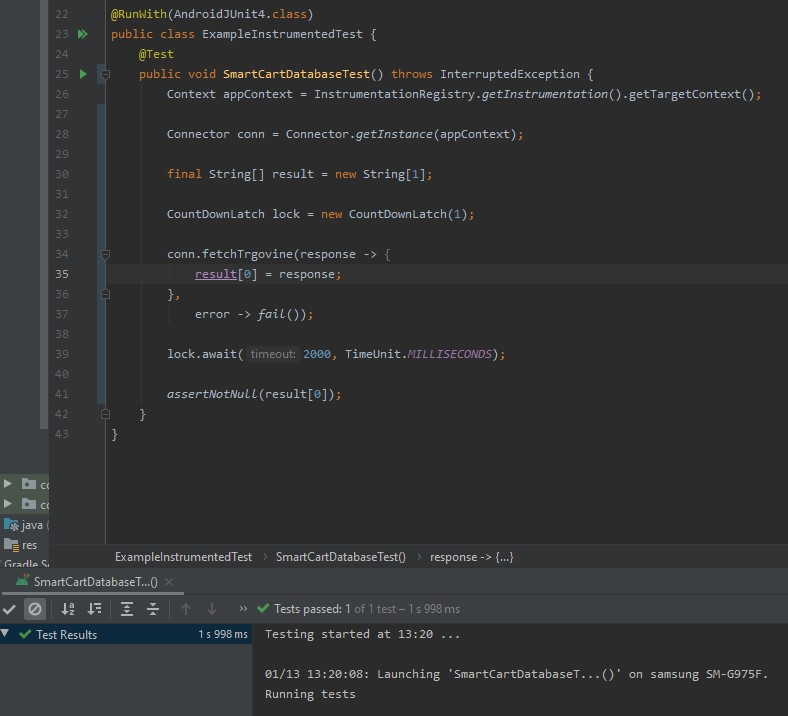
\includegraphics[scale=0.7]{slike/androidTest1.jpg}
				\caption{Testiranje baze podataka na uređaju}
				\label{fig:test_uredaj_db}
			\end{figure}
		
			\begin{figure}[H]
				\centering
				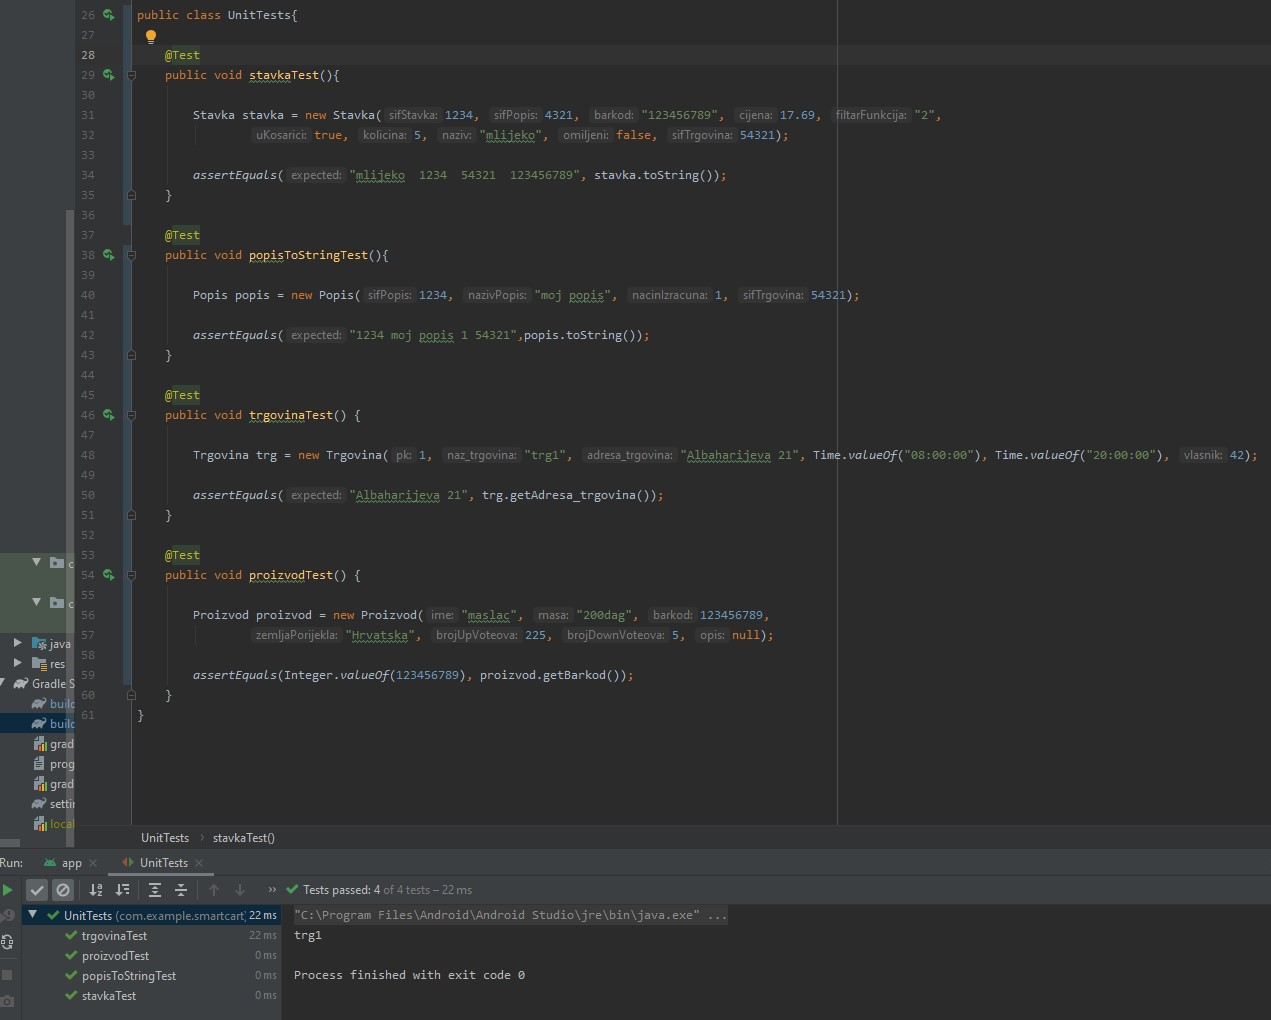
\includegraphics[scale=0.5]{slike/androidTest2.jpg}
				\caption{Testiranje razreda na uređaju}
				\label{fig:test_uredaj_class}
			\end{figure}
		
		\subsection{Ispitivanje sustava}
			
			Ispitivanje sustava je provedeno koristeći funkcionalnosti iz paketa unittest koji dolazi u instalaciji programskog jezika Python u kombinaciji sa alatom Selenium WebDriver koji pruža podršku za automatsko upravljanje internetskim preglednikom. Za instalaciju podrške za ispitivanje sustava potrebno je sa interneta skinuti Selenium za programski jezik Python (\url{https://pypi.org/project/selenium/}, također je moguće instalirati ako se unutar naredbenog retka pozove komanda \textit{pip install selenium}). Uz Selenium za Python potrebno je instalirati i Selenium WebDriver. U našem projektu koristimo geckodriver 0.28.0, verziju Selenium WebDriver-a za internetski preglednik Mozilla Firefox, koja se može skinuti sa sljedeće web-adrese: (\url{https://github.com/mozilla/geckodriver/releases/tag/v0.28.0}).\\
			Nad sustavom se provode razna testiranja. Neka od najvažnijih su:
			
			\begin{itemize}
				\item Testiranje izrade novog profila i pokušaja prijave na web-stranicu pomoću točne i krive kombinacije (relevantan isječak iz koda):
				\lstset{language=Python, tabsize=4, showstringspaces=false, basicstyle=\small}
				\begin{lstlisting}[breaklines]
def fill_login_form(self, username, password):
    self.driver.get(HOME_PAGE)
    self.driver.find_element(By.XPATH, '//button[text()="Log in"]').click()
    self.driver.find_element(By.NAME, "username").send_keys(username)
    self.driver.find_element(By.NAME, "password").send_keys(password)
    self.driver.find_element(By.NAME, "submit_button").click()
					
def test_successful_login(self):
    self.fill_login_form("ante@fer.hr", "pwd")
    self.assertEqual(self.driver.current_url, f"{HOME_PAGE}/trgovac")
					
def test_wrong_login(self):
    self.fill_login_form("ante@fer.hr", "abc")
    self.assertTrue(str(self.driver.current_url).startswith(f"{HOME_PAGE}/login"))
					
def test_create_new_profile(self):
    self.driver.get(HOME_PAGE)
    self.driver.find_element(By.XPATH, '//button[text()="Sign up as kupac"]').click()
    self.driver.find_element(By.NAME, "email").send_keys(NEW_USERNAME)
    self.driver.find_element(By.NAME, "password").send_keys(NEW_PASSWORD)
    self.driver.find_element(By.NAME, "confirm_password").send_keys(NEW_PASSWORD)
    self.driver.find_element(By.NAME, "submit_button").click()
    self.fill_login_form(NEW_USERNAME, NEW_PASSWORD)
    self.assertTrue(f"Logged in as {NEW_USERNAME}" in self.driver.page_source)	
				\end{lstlisting}
				\item Testiranje dodavanja novog proizvoda (relevantan isječak iz koda):
				\begin{lstlisting}[breaklines]
def test_adding_new_barcode(self):
	self.fill_login_form("ante@fer.hr", "pwd")
	self.driver.find_element(By.NAME, "barkod_artikla").send_keys(BARCODE)
	self.driver.find_element(By.NAME, "new_barcode_button").click()
	list_of_products = self.driver.find_element(By.ID, "products")
	self.assertTrue(BARCODE in list_of_products.text)
				\end{lstlisting}
				\item Testiranje „sigurnosti“ stranice (nepostojeći linkovi i pristup linkovima koji zahtjevaju posebnu dozvolu) (relevantan isječak iz koda):
				\begin{lstlisting}[breaklines]
def test_wrong_link(self):
	self.driver.get(f"{HOME_PAGE}/another_link/that_doesnt_exist")
	self.assertEqual(self.driver.current_url, f"{HOME_PAGE}/")

def test_page_permissions(self):
	self.fill_login_form(NEW_USERNAME, NEW_PASSWORD)
	self.driver.get(f"{HOME_PAGE}/trgovac")
	self.assertEqual(self.driver.current_url, f"{HOME_PAGE}/")
				\end{lstlisting}
			\end{itemize}
		
			Razultati testiranja:
			\begin{figure}[H]
				\centering
				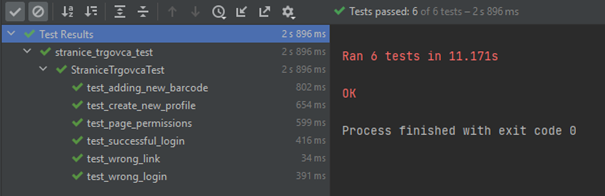
\includegraphics{slike/serverTest.png}
				\caption{Razultati testiranja servera}
				\label{fig:test_server}
			\end{figure}
		\eject
	\section{Dijagram razmještaja}
		Ovo treba napisati.
		\eject
	\section{Upute za puštanje u pogon}
		Ovo treba napisati.
		\eject
			